\chapter{多版本缓冲事务技术及文件系统效能优化}
\label{chap:vct}

\section{文件系统及效能优化}

\subsection{现有文件系统设计和页缓存}

\subsection{文件系统对应用效能的影响}

\subsection{数据一致性和滞后性}

\section{以内存为中心的文件系统}

\subsection{设计原则}

\subsection{系统架构}

\begin{figure}
  \centering
  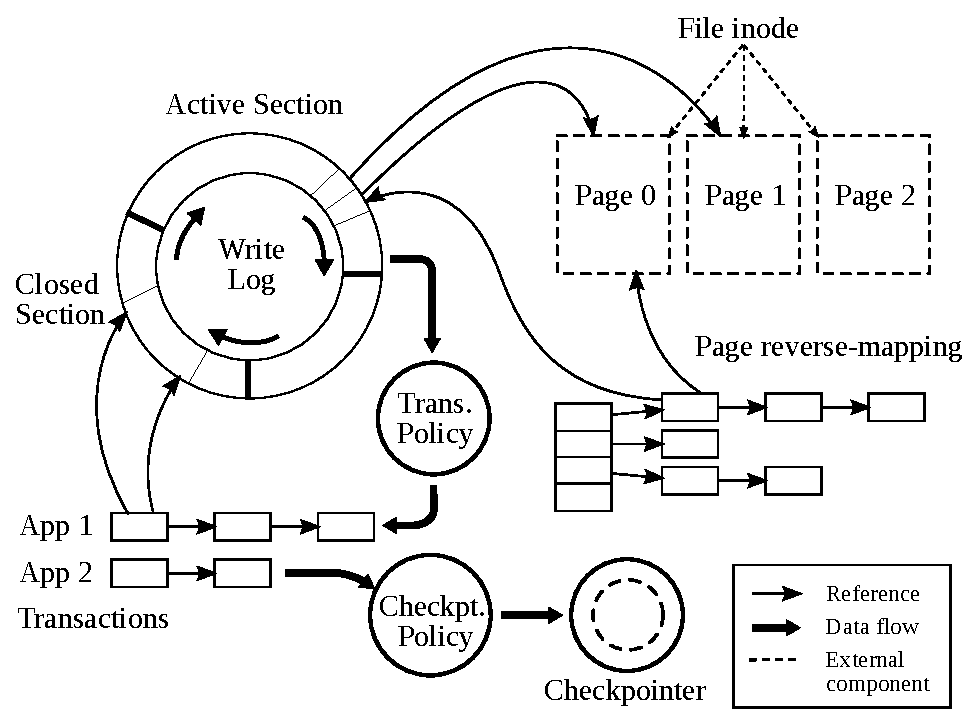
\includegraphics[width=0.8\columnwidth]{arch}
  \caption{MobiFS系统架构图}
  \label{fig:arch}
\end{figure}

MobiFS主要由五个模块构成:(1)页缓存,负责在内存中存储文件数据;(2)写日志,负责维护写操作的历史,由按序排列的许多记录项构成;(3)事务,写日志中的若干记录项归并为一组,它们的一致性不受覆写和重排序等优化的影响;(4)检查点生成器(checkpointer),负责调用底层闪存存储组件以原子性方式完成事务的持久化;(5)策略引擎,负责依据优化算法划分事务的边界,监听用户交互行为,并决定生成检查点的事务和时机。图~\ref{fig:arch} 描绘了MobiFS的系统架构。

MobiFS的设计充分考虑了与现有操作系统(Linux)的兼容和组件重用。它与操作系统共享现有的页缓存结构。对于页缓存的每个写操作,都会记入写日志,通常体现为在当前事务中(写日志的末尾)追加一个记录项,除非当前事务已经包含目标页地址的记录项。为此,我们需要维护一组从页地址到写日志项的逆向映射,以判断目标页地址是否已经存在于事务中。基于写日志和逆向映射,MobiFS建立起原子性事务机制。每个事务定义了可以进行覆写和重排序等优化的一个特定范围。最终,策略引擎指导检查点生成器保存事务到闪存,同时不影响用户交互。策略引擎根据每个手机应用甚至是用户的行为及其统计指标,做出动态的智能的判断。

在一个典型的配置中,不同手机应用会拥有自己独立的写日志和事务,但他们共享逆向映射、策略引擎和检查点生成器等组件。

\section{多版本缓冲事务技术}

\subsection{写日志}

\subsection{事务和版本}

\subsection{故障恢复}

\subsection{检查点生成}

\section{效能优化策略和算法}

\subsection{概述}

\subsection{事务划分算法}

\subsection{行为间隔预测}

\subsection{事务调度}

\section{系统实现和效能评测}

\subsection{系统实现}

\subsection{评测方法}

\subsection{内存占用评测}

\subsection{应用和用户感知评测}

\subsection{应用响应度评测}

\subsection{能耗评测}

\section{本章小结}

